\section{Illustrative Example Showing the Effects of Granularity}
To see how different representations of the system will alter the IVC and MinCutSet computations, let us examine a simple sensor example system. In this simple AADL architecture, the environmental temperature and pressure is sent to a subsystem of sensors which contains a temp sensor and a pressure sensor, both of which receive the respective environmental inputs. If the temperature (or pressure) surpasses a given threshold, then the temp (pressure) sensor outputs a HIGH\_LEVELS flag. It also outputs the temperature (pressure) reading seen at the sensor. A diagram showing the two levels of the AADL implementation is shown in Figure~\ref{fig:sensorGran1}.  

\begin{figure}[h]
\begin{center}
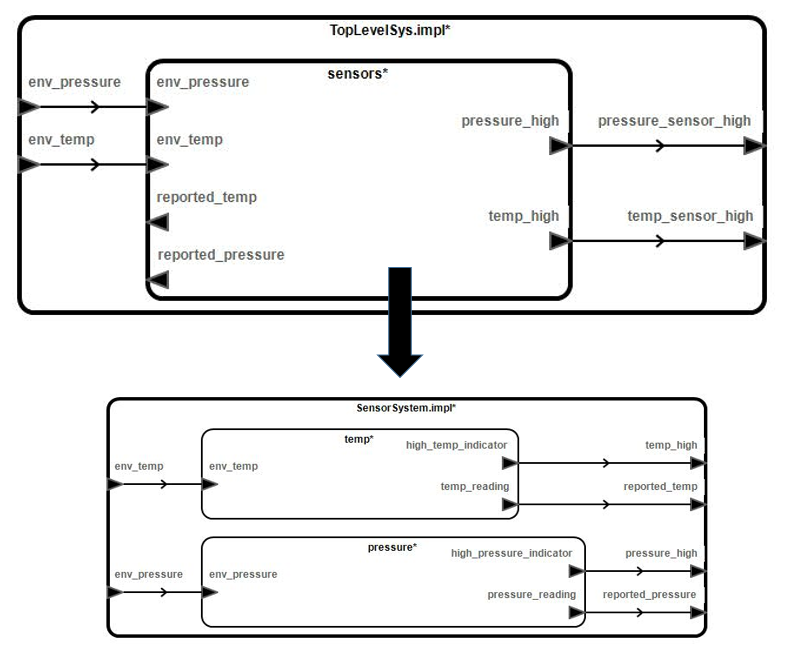
\includegraphics[width=14cm]{images/sensorGran.png}
\caption{Tempurature Sensor System} 
\label{fig:sensorGran1}
\end{center}
\end{figure}

Now that the basic architecture is in place, we focus our attention on the requirements of each component. The behavior we wish to enforce at the temperature sensor level corresponds to the following two guarantees, $G_1$ and $G_2$. (Note: pressure sensor behavior is quite similar and for this reason, we will stick to the temperature for this example.) 

$G_1$: If environmental temperature surpasses threshold, then output high temperature indication: \textit{(temp $>$ THRESHOLD) $\implies$ (high\_temp\_indicator)}

$G_2$: Temperature read is equivalent to temperature in\footnote{This example eliminated the possibility of noise in the temp reading for simplicity's sake.}: \textit{temp = temp\_reading} 


These can be seen in the model as two distinct guarantees over the output of the sensor component. Now, as the contracts work their way up the system, there are distinct ways of writing them. For this, we will look to two metaphorical engineers who will provide the higher layer contracts to us. 

Let us assume that system A is built by engineer A. The top level safety property states: 
\begin{center}
    \textit{If environmental temperature reaches 90 degrees, then system reports high temperature.}
\end{center}

The direct subcomponent is the sensor system which contains the outputs: (1) a high temp indicator, and (2) the actual temperature. Engineer A chose to write the supporting contract in the subsystem as follows: 
\begin{center}
    $(T \geq 90 \implies temp\_high) \land (temp\_indicator = T)$ 
\end{center}
  
The example temp sensor system contract hierarchy is shown in Figure~\ref{fig:granularityEx1}.  

\begin{figure}[h!]
\begin{center}
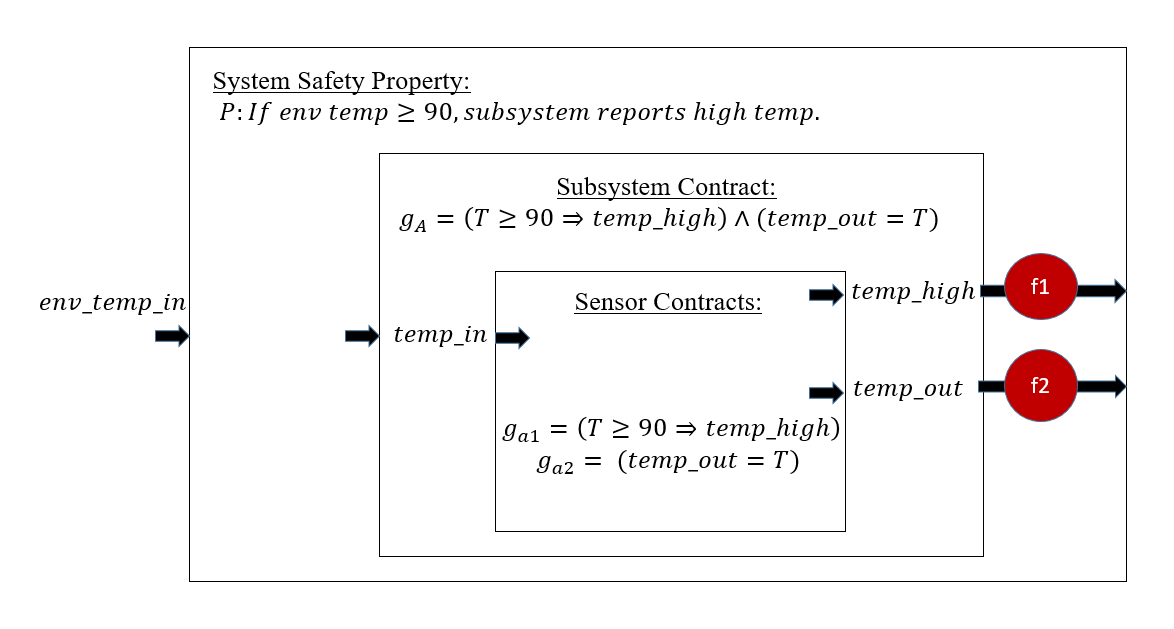
\includegraphics[width=10cm]{images/granularityEx.PNG}
\caption{Temp Sensor System Contract Part I} \label{fig:granularityEx1}
\end{center}
\end{figure}

The safety property at the top level requires the contract $g_A$ for proof of validity. Thus, the \aivcalg should contain the contract $g_A$ as an IVC. 

There are two faults defined for the temperature subsystem; one for each of the outputs. Fault $f_1$ affects the $temp\_high$ output and fault $f_2$ affects the $temp\_out$ output. Since each of these faults will violate the contract $g_A$, each of them should be found in the \textit{MinCutSet} for $G_A$.

Now assume that Figure~\ref{fig:granularityEx2} was the system contract representation built by engineer B. 

\begin{figure}[h!]
\begin{center}
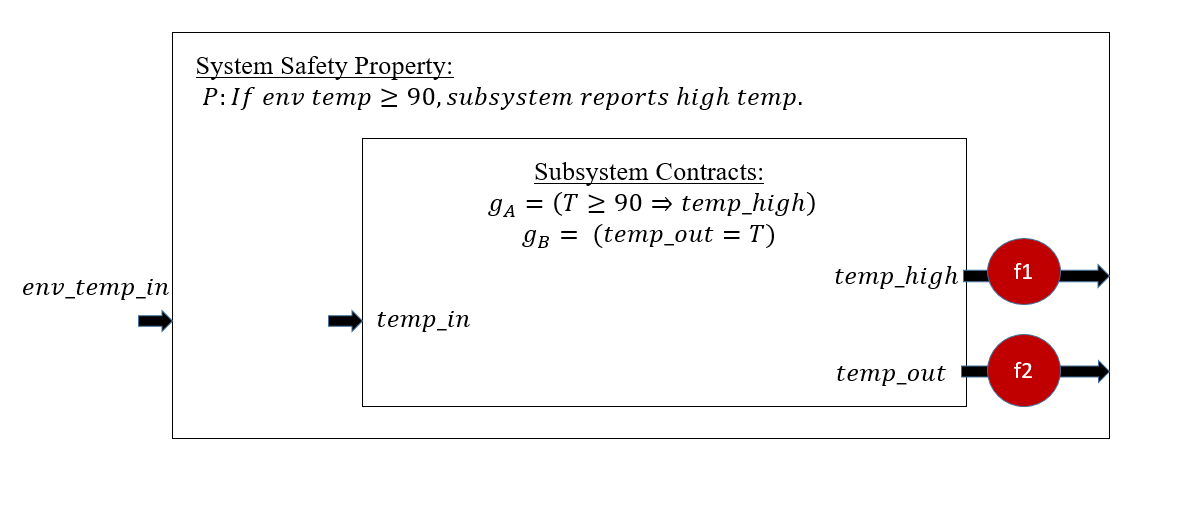
\includegraphics[width=10cm]{images/granularityEx2.PNG}
\caption{Temp Sensor System Contract Part II} \label{fig:granularityEx2}
\end{center}
\end{figure} 

The behavior and architecture of the system is the same, but the contract for the subsystem is more \textit{granular}; it is stated as two separate contracts:
\begin{center}
    $ g_A = (T \geq 90 \implies temp\_high)$ \\ 
    $ g_B = (temp\_indicator = T)$ 
\end{center}

Since $g_B$ is not required for the proof of the system safety property, only $g_A$ is found in the \textit{IVC}s and thus only $f_1$ will be seen in the \textit{MinCutSets} for this particular contract. 
 
In this simple example, it is easy to see how the granularity of the contracts may greatly affect the results of analysis.